\documentclass[a4paper,12p,titlepage]{article}
\usepackage[utf8]{inputenc}
\usepackage{listings}
\usepackage{amsmath}
\usepackage{graphicx}



\begin{document}

\begin{titlepage}
\title{6TRANSPERF\\
\normalsize Design, Implementation and Testing of a Benchmarking Program for the DS-Lite IPv6 Transition Technology}
\author{Alexandru Tiberiu Moise}
\date{February 2022}
\end{titlepage}
\maketitle
\tableofcontents
\newpage

\section{Summary}
Currently Internet is in a transition from IPv4 to IPv6. To facilitate the communication of these two incompatible versions of the Internet Protocol, IETF has defined a high number of IPv6 transition technologies, which have several different implementations. Their performance is an important decision factor for the network operators, when choosing the most suitable one of their purposes. 
IETF has defined a standard benchmarking methodology for the performance analysis of IPv6 transition technologies in RFC 8219. 6transperf aims to design, implement, test and document an RFC 8219 and RFC 4814 compliant Tester program for benchmarking the B4 and AFTR components of DS-Lite (RFC 6333).
6transperf is a single binary making use of Intel’s Data Plane Development Kit. It is relatively easy to customize, anyone wanting to add new packet formats to test different protocols can simply extend the existing classes which contain the logic for network buffer manipulation. Users of 6transperf can specify not only the transfer rate of the data stream but also the number of CPU logical cores responsible with data reception and transmission. Network interface cards implement multiple network buffer queues at the hardware level and typically an operating system will register an interrupt handler per CPU logical core, in the same fashion, DPDK is able to allocate multiple transmit/reception queues to use on the network interface card, and manipulate them as the user sees fit, the simplest configuration is to assign a logical core for each queue, therefore often there will be the case that half of the logical cores used by DPDK will be used to receive packets and the other half will be used to transmit packets. The main drive to use DPDK over the operating system network stack is the superior performance in terms of throughput and latency which comes from avoiding the inherent overhead of the packet stream passing through the network stack of the operating system. This overhead is due not only because of the userspace/kernelspace context switch but also, the network stacks of operating systems are designed to be as generic as possible, a great number of abstractions have been developed over the decades since the concept of having one computer communicate to another arose. These abstractions come at a cost, and for high capacity network interface cards the difference between using DPDK and not using DPDK can be in the order of tens of millions of frames per second. The below diagram shows some performance metrics of a regular layer 3 forwarding application based on DPDK and how it compares to the Linux network stack:

\begin{figure}[h]
\centering
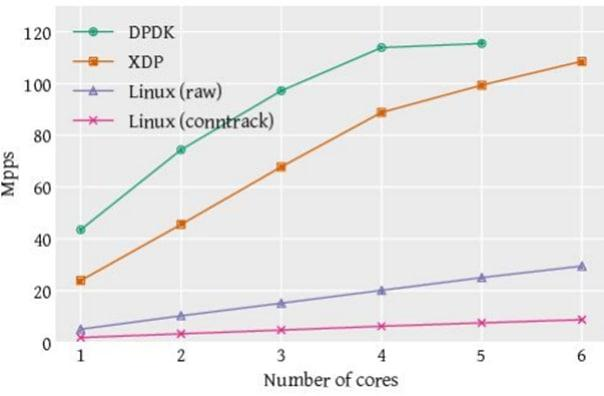
\includegraphics[width=\textwidth]{dpdk}
\end{figure}

\section{Introduction}
\subsection{What is DPDK and how does it work?}
DPDK is a collection of user space libraries which implements user mode network drivers that can be used by specialized networking applications which seek to avoid the overhead of the Linux kernel network stack. This is done by exposing the network interface’s PCIe endpoint resources such as the BAR registers, which are the interface between the device driver and the NIC hardware. In order to better understand how exactly DPDK interracts with network interface cards we will explain a bit about how PCIe endpoints are accessed in general:

\begin{figure}[h]
\centering
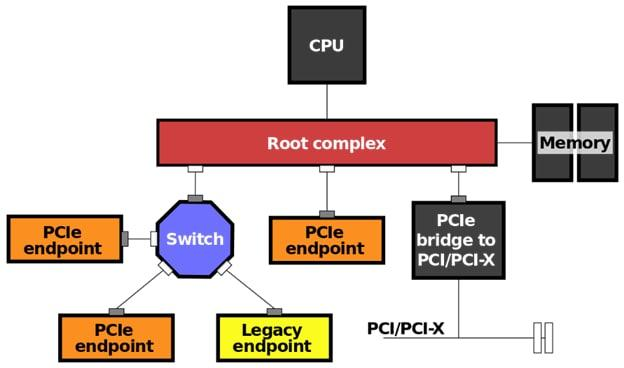
\includegraphics[width=\textwidth]{pcie}
\end{figure}

The above diagram serves to illustrate the high level view of a PCIe device tree starting from the root complex of a CPU and ending at the PCIe endpoints. In our case, our network interface card is such a PCIe endpoint. The PCIe bus implements its own packet based protocol and endpoints are accessed by the CPU (or other peripherals) through certain physical addresses which are pre-allocated by the BIOS, the BIOS in turn exposes these addresses to the OS typically through a set of fields describing the platform’s device tree structure within a table format which conforms with the ACPI standard.
Within this physical address space pre-allocated by the BIOS, any PCIe endpoint once connected will populate a data structures known as the "PCIe configuration space header", the format of this header is shown below:

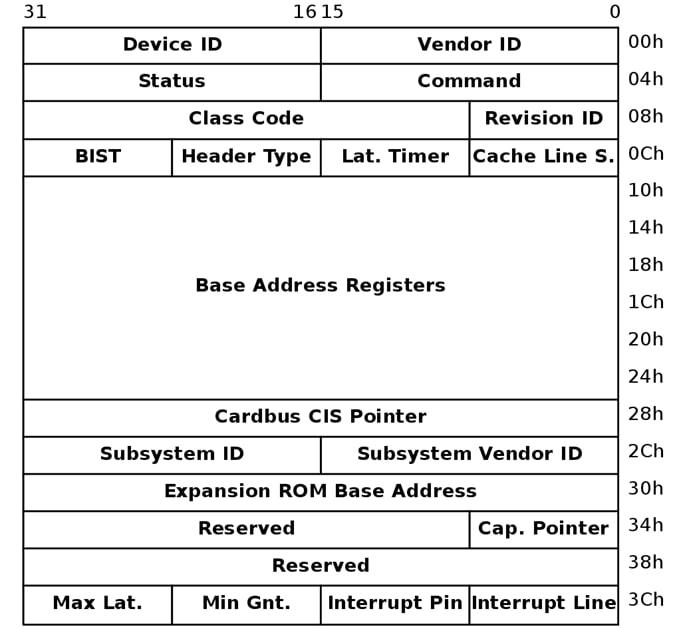
\includegraphics[width=\textwidth]{pcieconfig}

The Device ID and Vendor ID fields are typically the prime means for the Linux kernel to figure out which device driver should be matched against which PCIe endpoint. Other fields within this structure can be used to query the link layer connectivity status of the endpoint and issue link layer commands, such as a device-level reset. The Base Address Registers starting at offset 0x10 is where hardware manufacturers will expose all the internal registers of the PCIe endpoint, including the addresses of the transmission and reception queues of network interface cards, this is not necessarily the only means of configuration of a PCIe device, if one studies closely the electrical interface of a PCIe card one may find some additional pins leading to the System Management Bus interface of the CPU, which is a 2 wire interface similar to I2C. This is typically used as a sideband configuration interface by a device driver:

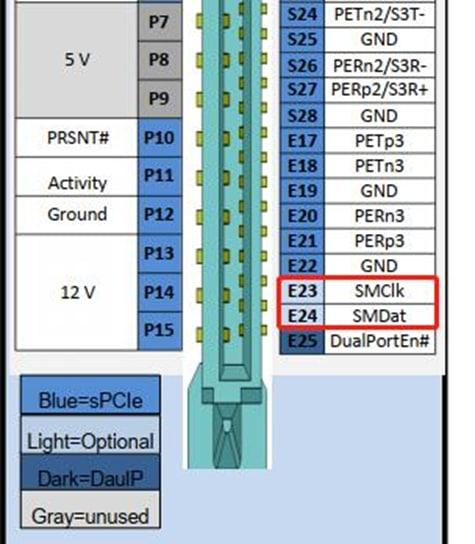
\includegraphics[width=\textwidth]{connector}

After explaining what exactly DPDK is accessing in order to interface with a network interface card, which is through the PCIe BARs, the next step would be to understand how it interfaces to the address space associated to the NIC: There needs to be a kernel level interface between the users pace application and the hardware, and that interface is called the "user space IO" subsystem (UIO). This device driver plays only the intermediary role of setting up virtual address mappings towards the physical resources, once these mappings are set, the application is able to copy data to and from the PCIe endpoint directly. The UIO kernel driver is also capable of delivering interrupts from the hardware endpoint to the user space application, the application listens for interrupts by issuing a blocking read() system call to a certain device file, the interrupt is known to have been received if/when the read() call returns execution to the caller. The below diagram illustrates the high level view of where a DPDK based application is situated from a functional perspective:

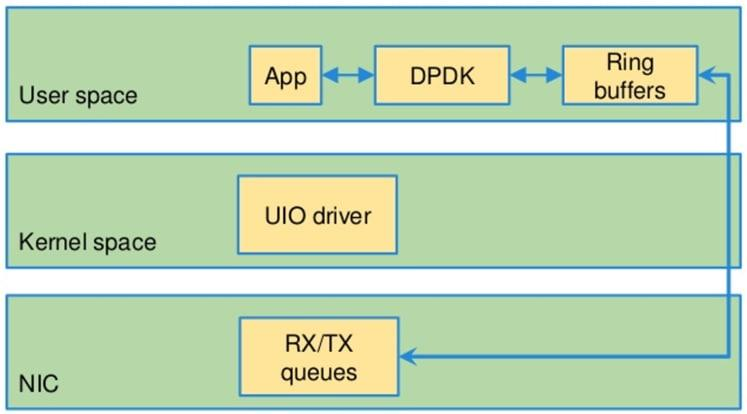
\includegraphics[width=\textwidth]{dpdkstack}

In order to make use of the UIO driver, it must first be attached to a certain PCIe endpoint. The Linux kernel provides nodes into the sysfs filesystem which can be used to easily detach and re-attach drivers manually to any external device. DPDK provides scripts which makes it easier to attach any UIOuio kernel modules to our PCIe endpoints, for example, if we wish to add two ports from a dual port NIC to the DPDK environment, we simply execute the following commands:

\begin{lstlisting}
dpdk-devbind --bind=uio_pci_generic 0000:03:00.0
dpdk-devbind --bind=uio_pci_generic 0000:03:00.1
\end{lstlisting}

 Once the UIO driver is attached, a number of "/dev/uioN" nodes will appear in the devfs filesystem, one node for each PCIe resource. In order to access the PCIe address space through the uio UIO device, an application simply needs to use the mmap() system call to create an association between a virtual address within the process address space and a physical address associated with the PCIe endpoint which is exposed by the UIOuio driver. The mapping of these devices is handled by DPDK internally and DPDK users do not need to worry about this implementation detail. Generally the only configuration parameters pertaining to the NIC hardware are those of functional nature with respect to the data handled, such as number of queues, which hash function should be used, receive side scaling, and so on. These are parameters that the Llinux kernel would also expose to user space either via sysfs nodes or the ethtool interface.

\subsection{What is DS-Lite?}

Defined by RFC6333, Dual-Stack Lite is an IPv6 transition technology which aids internet service providers to migratde their network to IPv6 without requiring any modifications from the customer side., Ffrom their perspective, there is no difference between connecting directly to the IPv4 internet or connecting to it via an IPv6 tunnel. At the same time any customers using IPv6 are able to connect directly to IPv6 internet, when an internet service provider uses the DS-Lite technology.

All implementation of DS-Lite follow the following formula:

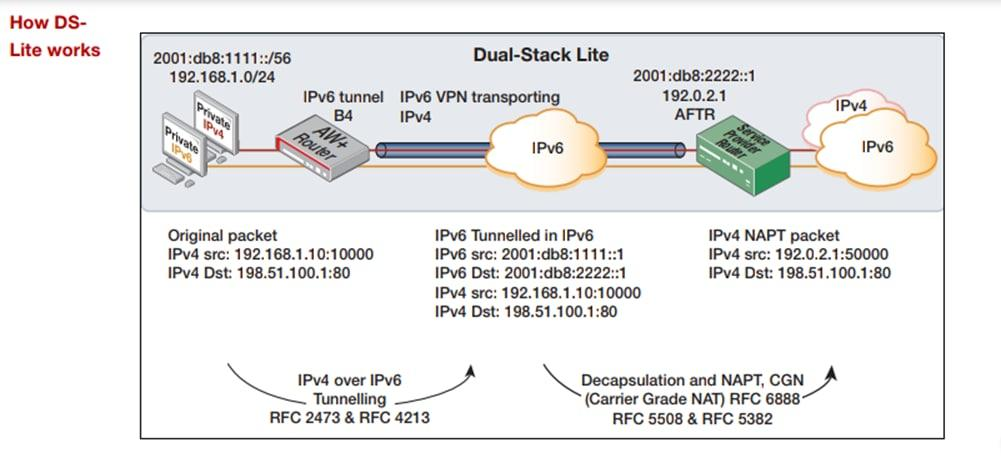
\includegraphics[width=\textwidth]{dslitehighlevel}

There are two elements in the DS-Lite technology, the Basic Bridging BroadBand element (hereafter knowon as the "B4" element), and the Address Family Transition Router element (hereafter known as the "AFTR" element). The B4 element can be implemented by any IPv4 and IPv6 capable router that is facing the IPv6 internet. The B4 component performs the encapsulation of all IPv4 traffic originating from the internal network. Within it there is also an IPv6 tunnel, which is set up between the B4 and the AFTR components. Regular IPv6 traffic originating from the customer network bypasses this tunnel and goes directly towards the IPv6 internet. The function of the AFTR component is to perform the IPv6 tunnel decapsulation and afterwards to perform Network Address Translation (NAT) on the inner IPv4 packets towards the IPv4 internet.
The advantage of this approach is that there is no protocol family translation involved at all, and for the IPv4 only hosts behind the B4 router, the tunnel between the B4 and the AFTR elements is completely transparent.
The implementation of the AFTR element can be any router that implements an IPv4-in-IPv6 tunnel endpoint that is also capable of performing IPv4 to IPv4 NAT. At this point in time RFC6333 only defines IPv4-in-IPv6 tunnels however it is not excluded that in later revisions more encapsulation methods will be added. Our implementation of DS-Lite at the present moment is only capable of operating with IPv4-in-IPv6 tunnels.

\subsection{Design and implementation of the 6transperf DS-Lite B4 tester}
General considerations:
\subsubsection{Scope of 6transperf}
RFC8219 defines a methodology for testing the performance of IPv6 transition technologies. The five main measures of performance that 6transerf shall focus on are Throughput, Latency, Packet Delay Variation, Inter-Packet-Delay variation and Frame Loss Rate, it is also an end goal to run all the aforementioned tests both using transmission of single frames and back-to-back frames.
Whereas the initial implementation of 6transperf focuses on the DS-Lite IPv6 transition technology, 6transerf intends to be implemented in a generic way so that it may be easily extended to support other technologies alongside DS-Lite. It is for this reason that the C++ programming language has been used to take full advantage of the level of abstraction offered by its native support of the Object Oriented Programming paradigm.
\subsubsection{Performance considerations}
Due to the requirements of a tester to be able to send traffic both at a high and at a fixed number of frames per second towards a DUT it has been decided that 6transperf shall be implemented to use DPDK. As a reference there exist tables of theoretical rates for various Ethernet interface types for each given frame size, RFC5180 for example calculates these frame rates using the following formula given a frame size "X":

\begin{equation}
\frac{Line rate (bps)}{8 bits per byte*(X+20) bytes per frame}
\end{equation}

RFC8219 contains a similar table based on the one found in RFC5180, however the above formulas is adapted to also account for a certain frame size overhead, denoted as “O” in the denominator:

\begin{equation}
\frac{Line rate (bps)}{8 bits per byte*(X+O+20) bytes per frame}
\end{equation}

If one is to calculate the recommended frame rates for 6in4 encapsulation for example O is equal to 20, whereas a 4in6 tunnel, as is the case of DS-Lite, the overhead is equal to 40 bytes which is the size of the outer IPv6 packet.

\subsubsection{High-Level Implementation Decisions:}
\subsubsection{Software Architecture and Hardware Requirements}

RFC8219 requires bidirectional traffic to be ran during all measurements. 6transperf shall allocate a dedicated logical core for each allocated transmit and for each allocated receive queue. It is generally expected that the number of transmit and receive queues to be equal but that may not necessarily always be the case. As the previous statement suggests, a user should be able to allocate an arbitrary number of queues having as an upper bound either the number of logical cores the user has at their disposal, or the number of queues supported by the NICs physical hardware.

Using multiple receive queues may not always provide the best performance however since it has been found early on that many off-the-shelf Ethernet adapters may lack hash functions used in Receive Side Scaling (the hardware-based process of interrupt distribution internal to the NIC’s hardware) that are able to differentiate between different flows within the same IP tunnel, as such, the traffic specific to a particular tunnel may be resolved to a single hardware queue upon reception regardless of the inner part of the tunneled packet. Nevertheless, in order for 6transperf to be future proof, it is the intention that the queue allocation and partitioning be kept as a configurable parameter. In the simplest case, 1 transmit and 1 receive core shall be allocated per port adding to a total of 4 dedicated cores for the traffic, if we are to double the number of queues used then in turn the number of cores required to set aside shall also be doubled, as in he case of 2 TX/RX queue pairs requiring a total of 8 dedicated cores in order to run the traffic.

Both the Tester and the DUT must use two ethernet ports, referred to simply as “port 0” and “port 1”. A third interface is also preferred to be available to serve as the control/management interface towards both the DUT and the Tester.

\subsubsection{Input and Output}

As can be noted in the chapter above there is a separation between generating/processing the test results, which is performed by the 6transperf binary and is implemented using C++, and the presentation/interpretation alongside validation of these results. The latter of the two shall be implemented using a bash script implementing a binary search tree algorithm in order to identify the highest rate the tester is able to send where no frame drops occur. An example of such a script which may be used as a reference is present in the stateless NAT64 tester “siitperf”. At the end of the execution the same script is expected to consolidate the results of each testrun into a coherent whole, conforming to the table format described in RFC8219.
Non-fixed parameters such as frame size, frame rate, number of queues, logical core allocation, which type of tests are to be run shall all be specified via command line arguments to the 6transperf binary. These arguments shall be calculated programmatically and supplied by the higher-level script mentioned above, this also means that the script shall execute multiple runs of 6transperf. Fixed parameters such as IP addresses, MAC addresses, tunnel configurations, shall be stored in a local configuration file. 6transperf shall provide results that are relevant to the testing script’s decision-making process in an easily parse-able format to the standard output. The test script shall parse these results using standard Linux command-line tools such as “sed”,”grep” and “awk”. 6transperf may also output to a file more verbose results that are not relevant for the decision making process of the test script as it sees fit.

\subsubsection{Implementation of the Tests}
\subsubsection{General considerations and Input parameters}

All the supported measurements are implemented by one binary, and different parameters to the binary shall run different types of tests for different technologies. The full range of the command line arguments that 6transperf supports and all possible combinations of these parameters shall be output to the standard output before immediately exiting if 6transperf is ran without it being supplied any parameters. Although RFC8219 considers the throughput, latency, pdv, ipdv and frame loss rate to be separate tests, generally all tests will report the throughput and frame loss rate for any given configuration of the tester. 6transperf uses positional command line parameters, the ones common to all tests being:

\begin{itemize}
\item Frame size (in bytes), this shall be the frame size minus the overhead, as the overhead can be different for each port depending on the configuration, as one port may be sending IPv4 frames while the other is sending 4in6 encapsulated frames for example.


\item Frame rate (in frames per second)

\item Test duration (in seconds)

\item RX Delay (in seconds) this parameter controls the window of time in which we continue to run the receive side threads after the transmit side threads have ended their execution, this is to give time for all packets on the NIC’s receive buffers to be processed.

\item TX Delay (in seconds) this parameter adds a waiting period between the NIC initialization and the transmission loop. It has been observed that even though the init function of the network driver may return, the actual hardware may not be able to transmit any traffic, thus causing packets to accumulate at the beginning of the test, and thus a spike at the beginning of the packet stream.
\end{itemize}

\subsection{Types of measurements:}
\subsubsection{Throughput and Frame Loss Rate Measurements}

6transperf transmits a fixed number of frames within a given timeframe (specified in seconds via the -duration parameter). The results are reported on a per-port basis, ports are 0-indexed and they are ordered according to the natural ordering used by the DPDK library, which is to enumerate network cards in the order in which the appear in the PCIe tree.

The tester will report the results in the given format:

\begin{lstlisting}
Port 0 total:
rx: 120000000 frames (7680000000 bytes, 61440000000 bits)
tx: 120000000 frames (7680000000 bytes, 61440000000 bits)
Port 1 total:
rx: 120000000 frames (7680000000 bytes, 61440000000 bits)
tx: 120000000 frames (7680000000 bytes, 61440000000 bits)
Port 0 dropped frames: 0(0%)
Port 1 dropped frames: 0(0%)
\end{lstlisting}

In the above example we have sent 2 million packets per second for the duration of 60 seconds. After the absolute values of the transmitted and received number of packets, the number of dropped frames per port is reported both as the actual number of packets lost, and as a percentage of the total number of packets transmitted for that port.
The test shall be considered successful if no frame loss occurs, the tester itself does not consider any of its results to be either successful or not, interpretation of the results is to be performed by a higher level script such as the one used to perform a binary search after the maximum no-drop rate the tester is capable of.

\subsubsection{Latency measurements:}

This test is selected by providing the (--lat) command line parameter to 6transperf. According to the guidelines set by RFC8219, 6transperf will not tag any latency frames at the beginning of the timeframe in which traffic is running. A delay parameter shall be specified and subtracted from the total test duration, after this period has elapsed, the latency frames shall be distributed uniformly across the remaining traffic, the latency frames shall be tagged with a certain numeric identifier at a specific offset within the packet in order to distinguish them from other test frames. The send and receive timestamps are taken right after sending the packet on the wire, and immediately after receiving. All latency frames carry within them sequence numbers that are to be used to index into the array keeping the timestamps and match each TX timestamp with its corresponding RX timestamp. The results of this test come in the following form:

\begin{lstlisting}
Port 0 median latency: 0.032736 msec
Port 0 worst-case latency: 0.111738 msec
Port 1 median latency: 0.032474 msec
Port 1 worst-case latency: 0.109170 msec
\end{lstlisting}

The median and worst-case latency are reported for each port in milliseconds. The results are only meaningful if 0% frame loss occurred for each given port. If frame loss occurs then 6transperf is expected to perform the same binary search algorithm that was used during the throughput test to find the max no-drop rate of the medium.

\subsubsection{PDV}

The test is selected by providing the (--pdv) command line parameter to 6transperf. The manner in which frames are tagged and timestamped is similar to the latency measurement, except that in this case all frames shall be tagged with a sequence ID and no special identifier shall be required to distinguish the timestamped frames from any other frames since all frames are supposed to be timestamped. The results are reported per port as in the case of all other tests:

\begin{lstlisting}
Port 0 PDV: 0.113127 msec
Port 1 PDV: 0.113641 msec
\end{lstlisting}

\subsubsection{IPDV}

This test is selected by providing the (--ipdv) command line parameter to 6transperf. As in the case of the PDV test, every frame will be timestamped, except that the differences between the delays of each 2 consecutive packets is compared and what is reported is the min, median and max IPDV:

\begin{lstlisting}
Port 0 Min IPDV: -0.181530 msec
Port 0 Median IPDV: -0.000010 msec
Port 0 Max IPDV: 0.155866 msec
Port 1 Min IPDV: -0.140553 msec
Port 1 Median IPDV: -0.000012 msec
Port 1 Max IPDV: 0.188056 msec
\end{lstlisting}

\subsection{Configuration:}

%The only role of the config_file is to configure the mac, ip4/6 addresses, and to select which one of the two ports shall be used as the tunnel interface. If the port is selected as a tunnel interface, then the construct_ipip6_packet method will be used on that port and it will construct a packet with an outer ip6 header containing the below given ip6 address, with the inner ip4 header containing the address specified in the config_file for the given port.

Below is a sample configuration:

\begin{lstlisting}
b4_port0_mac_self=a0:36:9f:13:fe:28
b4_port1_mac_self=a0:36:9f:13:fe:2a
b4_port0_mac_peer=a0:36:9f:13:e5:38
b4_port1_mac_peer=a0:36:9f:13:e5:3a

b4_port0_ip_self=200.1.2.3
b4_port0_ip_dest=168.196.2.1
b4_port1_ip_self=168.196.2.1
b4_port1_ip_dest=200.1.2.3

b4_port0_ip6_self=2001:2:0:0:0:0:0:3
b4_port0_ip6_dest=2001:2:0:0:0:0:0:2
b4_port0_tunnel=yes
\end{lstlisting}

\subsection{Implementation Details}
\subsubsection{Time Handling}

The timing logic is based on the intel x86 RDTSC instruction. There may exist certain concerns with regards to synchronization across the TSC  registers between different physical CPUs, therefore all tests ran by 6transperf assume that all logical core used by DPDK run on the same physical CPU.

\section{Description of the test setup}
The test setup consists of two separate hosts, one is the Tester, the other is the Device Under Test, between the two there are two network interfaces, each host’s interface is connected to the corresponding interface of the other, below there is a drawing, taken from RFC 8219 exemplifying this setup:

\begin{lstlisting}[basicstyle=\tiny]







                           +--------------------+
                           |                    |
              +------------|IPvX   Tester   IPvY|<-------------+
              |            |                    |              |
              |            +--------------------+              |
              |                                                |
              |            +--------------------+              |
              |            |                    |              |
              +----------->|IPvX     DUT    IPvY|--------------+
                           |                    |
                           +--------------------+

\end{lstlisting}

The physical setup will require 6transperf to be executed on a server which has a much higher performance capability than the router we are testing, this is required because if we are to test the B4 and AFTR elements at their highest bounds we require the capability to send traffic beyond what the router can handle. In the below diagram the physical setup between the Tester and the DUT can be seen:

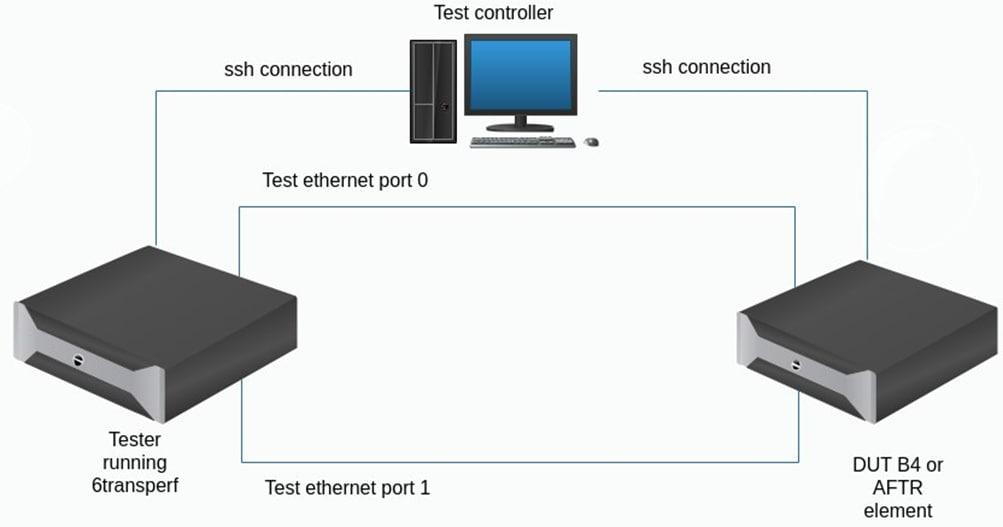
\includegraphics[width=\textwidth]{testsetup}

As can be seen above, a typical physical setup includes the Tester, the DUT, with 2 high speed ethernet connections shared between them. A side interface on each device is reached from a controller, typically via a SSH connection.
6transperf will expect to be assigned two separate physical ports for each side of the tester. Depending on the tester configuration, it is either capable of sending IPv4-only, IPv6-only or IPv4-in-IPv6 frames. These frames carry with them an identifying tag so that they can be distinguished from any other traffic that may be present on the wire, this way only the traffic generated by the tester will be accounted for, when calculating or reporting any results.
The physical systems (hereafter referred to as N-Nodes) used that have been provided are two identical Dell PowerEdge C6220 servers in the NICT StarBED, Japan. They were equipped with two 2GHz Intel Xeon E5-2650 CPUs having 8 cores each, 128GB 1333MHz DDR3 RAM and Intel 10G dual port X520 Ethernet network adapters. The Debian Linux operating system was updated to version 9.13 on all computers. The Linux kernel used by the tester machine is a 5.3.9 kernel which was custom compiled with a number of CPU scheduler-specific optimizations that serve to benefit a DPDK environment in which only a single application will generally have a CPU core for itself. This being the case we can take the liberty for example of disabling timer interrupts on the DPDK cores so that the timer interrupt handlers for those CPU cores will not interfere with the DPDK cores. This can be accomplished by setting the $$"CONFIG\_NO\_HZ\_FULL=y"$$ kernel configuration parameter before compiling the kernel, and listing the CPUs which should be excluded from handling timer interrupts via the $$nohz\_full=<cpus>$$ kernel boot command line parameter. It’s also generally good practice when operating a tester to lock the CPU frequency to the highest base frequency available so that the variation due to CPU execution time can be minimized. This can also be accomplished via certain sysfs nodes related to the "cpufreq" driver in the Linux kernel.

\subsection{B4 implementations to be tested:}
The greatest difficulty about this is that there are many proprietary router vendors out there, such as Cisco, Juniper, Ericsson, Arista, etc. Most vendors will explicitly provide support for DS-Lite and offer sample configurations for how to configure their equipment either as a B4 or an AFTR router.
For cost saving reasons, we will restrict our scope to open source DS-Lite implementations.
Below we list a few the most used open source and proprietary DS-Lite implementations:

\begin{lstlisting}[basicstyle=\tiny]
1.	Configure manually ipip6 tunnel in Linux.

2.	OpenWrt: https://openwrt.org/docs/guide-user/network/ipv6_ipv4_transitioning#protocol_dslite_dual-stack_lite

3.	Lightweight 4over6 https://blog.apnic.net/2018/06/28/lw4o6-one-step-further-than-dual-stack-networks/

4.	Configuring DS-Lite on Juniper routers https://www.juniper.net/documentation/en_US/release-independent/nce/topics/example/ipv6-access-ds-lite-configuring.html

5.	Citrix ADC appliance DS-Lite configuration https://docs.citrix.com/en-us/citrix-adc/current-release/citrix-adc-support-for-telecom-service-providers/dual-stack-lite.html

6.	Allied Telesis DS-Lite configuration https://www.alliedtelesis.com/sites/default/files/documents/feature-guides/ds-lite_feature_overview_guide.pdf

7.	F5 BIG-IP CGNAT based DS-Lite https://techdocs.f5.com/kb/en-us/products/big-ip_ltm/manuals/product/cgn-implementations-11-5-0/14.html

8.	Huawei NE40E are advertised to support DS-Lite processing https://support.huawei.com/enterprise/en/doc/EDOC1100055020/501a998b/overview-of-ds-lite

9.	Cisco routers support DS-Lite configurations https://community.cisco.com/t5/ipv6/need-configuration-example-for-ds-lite-tunneling-ipv4-ipv6-nat44/td-p/2096112

10.	BSD-based systems using pfsense are capable of acting as a B4 router https://forum.netgate.com/topic/96702/state-of-ds-lite-dual-stack-lite-support-in-pfsense/10

11.	TP-Link native firmware supports DS-Lite https://static.tp-link.com/res/down/doc/TD-8816(UN)_V8_UG.pdf

12.	Mikrotik ROS v7beta release is supposed to support DS-Lite https://forum.mikrotik.com/viewtopic.php?t=154248
\end{lstlisting}

\subsubsection{Setting up a minimal B4 router using an ipip6 tunnel:}

The below diagram illustrates the physical setup of the DUT and Tester and their port configurations:

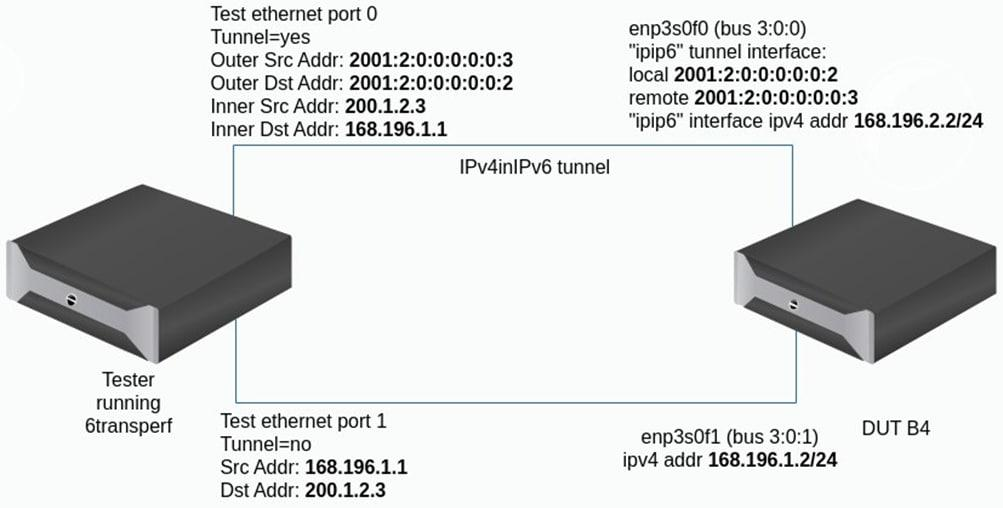
\includegraphics[width=\textwidth]{minimal}

To setup an ipip6 tunnel in Linux is a relatively straightforward process, below is a step by step explanation of how to set up an ipip6 tunnel that can be tested with 6transperf:

The N-nodes in the StarBED environment all have identical PCIe trees, and the NICs are wired in such a way that the port corresponding to the $$"3:00.0"$$ PCIe endpoint on the B4 element will be connected directly to the port corresponding to the $$"3:00.0"$$ PCIe endpoint of the tester.

First we may set up a tunnel interface and attach it to the Ethernet port corresponding to PCIe endpoint 3:00.0, the bus:device:function designation can be queried using the ethtool Linux tool:

\begin{lstlisting}
# ethtool -i enp3s0f0 | grep bus
bus-info: 0000:03:00.0
\end{lstlisting}


A tunnel interface can be created via the "ip link" command, part of the iproute2 Linux package. The below command shall create a tunnel interface named "ipip6", the outer source address of packets leaving this interface shall have address 2001:2::2, and it will be decapsulating all incoming packets on enp3s0f0 with outer source address 2001:2::3.

\begin{lstlisting}
# ip link add name ipip6 type ip6tnl local 2001:2:0:0:0:0:0:2 remote 2001:2:0:0:0:0:0:3 mode any dev enp3s0f0
\end{lstlisting}

The next step is to add an IPv4 address to the tunnel interface, this shall be used to route any IPv4 traffic through the tunnel interface.

\begin{lstlisting}
# ip addr add 168.196.2.2/24 dev ipip6
\end{lstlisting}

The IPv6 address which is assigned to the ipip6 tunnel must be assigned to the physical interface that the tunnel interface is attached to:

\begin{lstlisting}
# ip -6 addr add 2001:2:0:0:0:0:0:2/64 dev enp3s0f0
\end{lstlisting}

Next, we bring up the two Ethernet ports connected to the tester and the ipip6 virtual interface:

\begin{lstlisting}
# ip link set dev enp3s0f0 up
# ip link set dev enp3s0f1 up
# ip link set dev ipip6 up
\end{lstlisting}

We treat the interface corresponding to endpoint 3:00.1 as a regular IPv4 interface, this would be the port connected towards the customers network.

\begin{lstlisting}
# ip addr add 168.196.1.2/24 dev enp3s0f1
\end{lstlisting}

We will configure the "port1" 3:00.1 interface of the tester to send traffic towards IP address 200.1.2.3, which we consider to be some machine accessible via the internet, in order to simulate this we add a static route to the ip address 200.1.2.3 via the tunnel interface IPv4 address.

\begin{lstlisting}
# ip route add 200.1.2.3 via 168.196.2.2
\end{lstlisting}

6transperf does not have an ARP implementation, therefore it will ignore any ARP broadcast messages asking for which MAC address is associated to a certain IPv4 address, therefore, we are required to add a static ARP entry for the port1 IP address of the tester.


\begin{lstlisting}
# arp -s 168.196.1.1 a0:36:9f:13:fe:2a
\end{lstlisting}

The same must be done to the IPv6 address of port0 of the tester, IPv6 does not use ARP protocol for associating MAC addresses with IP addresses, a subset of ICMP is used called "Neighbor Discovery" instead, the neighbor table entries in the Linux kernel can be manipulated via the "ip -6 neigh" subcommand of the iproute2 package:

\begin{lstlisting}
# ip -6 neigh add 2001:2::3 lladdr a0:36:9f:13:fe:28 dev enp3s0f0
\end{lstlisting}

We also want that the B4 element will forward packets between the tunnel port and the port directed towards the customer networks, this is enabled via the following sysctl switch:

\begin{lstlisting}
# sysctl -w net.ipv4.ip_forward=1
\end{lstlisting}

Without having yet described the format of 6transfperf’s configuration file, it is not difficult to understand the below example configuration that allows 6transperf to communicate with the B4 element configured above:
First the destination and source addresses of the packets leaving each port must be statically  configured:

\begin{lstlisting}
b4_port0_mac_self=a0:36:9f:13:fe:28
b4_port1_mac_self=a0:36:9f:13:fe:2a
b4_port0_mac_peer=a0:36:9f:13:e5:38
b4_port1_mac_peer=a0:36:9f:13:e5:3a
\end{lstlisting}

After which the same must be done with the IPv4 and IPv6 addresses, note that only port0 is assigned an IPv6 address in the configuration below, because it is the only port that is to be configured as a tunnel interface:

\begin{lstlisting}
b4_port0_ip_self=200.1.2.3
b4_port0_ip_dest=168.196.1.1
b4_port1_ip_self=168.196.1.1
b4_port1_ip_dest=200.1.2.3
b4_port0_ip6_self=2001:2:0:0:0:0:0:3
b4_port0_ip6_dest=2001:2:0:0:0:0:0:2
b4_port0_tunnel=yes
\end{lstlisting}

\subsection{Software architecture of 6transperf:}
The base architecture is formed by 3 base classes. Tester, PortConfig and Port. Any newly added tester will be a subclass of Tester, as is the case for DSLiteTester.

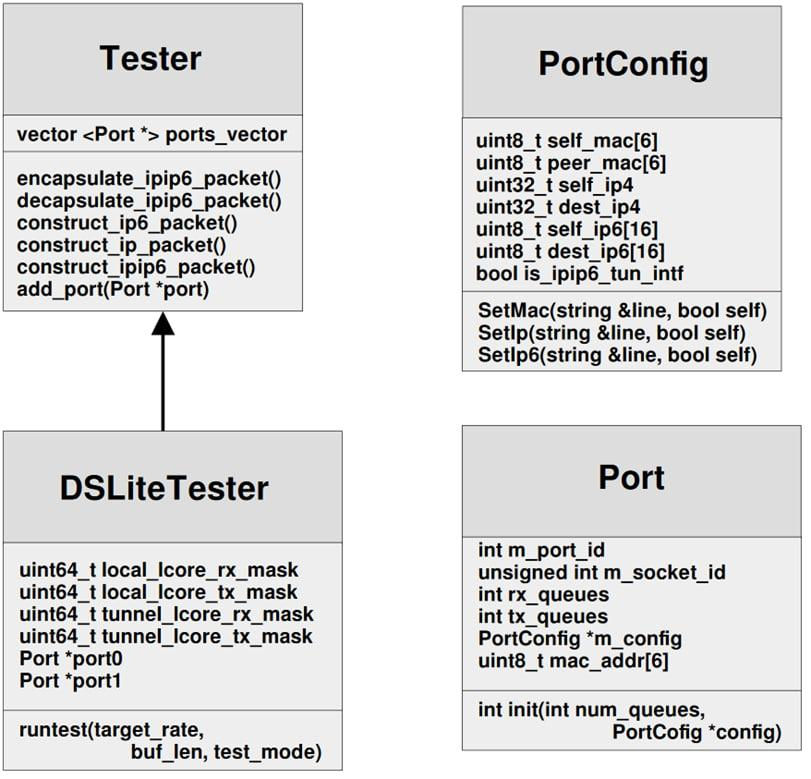
\includegraphics[width=\textwidth]{classdiagram}

The Tester class contains generic packet manipulation methods, such as those related to encapsulating/decapsulating a packet, or constructing an IPv4, IPv6 or pre-encapsulated packet. 

\begin{frame}

\lstset{language=C++,breaklines=true,numbers=left}
\begin{lstlisting}
class Tester
{
public:
        vector<Port *> ports_vector;
        //TODO: Must support more lcores than 64
        uint64_t port0_lcore_mask = 0;
        uint64_t port1_lcore_mask = 0;
        struct queue_stats *port0_stats;
        struct queue_stats *port1_stats;
        uint64_t num_tsc_pairs_per_qp;
        // one index per RX queue
        uint64_t *port0_tsc_pairs_index;
        uint64_t *port1_tsc_pairs_index;
        struct timestamp_pair **port0_tsc_pairs_array;
        struct timestamp_pair **port1_tsc_pairs_array;
        bool timestamp_all_packets = false;
        bool timestamp_500_packets = false;

        // When this counter is equal to the number of total rx queues
        // tx threads will start
        std::atomic<int> rx_ready_counter {0};

        void encapsulate_ipip6_packet(PortConfig *config, char *buf, int buf_len);
        void decapsulate_ipip6_packet(PortConfig *config, char *buf);
        void construct_ip6_packet(PortConfig *config, char *buf, int buf_len, bool timestamp_all_packets);
        void construct_ip_packet(PortConfig *config, char *buf, int buf_len, bool timestamp_all_packets);
        void construct_ipip6_packet(PortConfig *config, char *buf, int buf_len, bool timestamp_all_packets);
        virtual void set_lcore_allocation(uint64_t port0_mask, uint64_t port1_mask) { }
        virtual void set_ports_from_config(void) { }

        void add_port(Port * port);

        virtual ~Tester() = default;
};
\end{lstlisting}
\end{frame}

The "ports\_vector" is a collection of ports supplied to 6transperf via command line, there’s no logic into the Tester class about what the purpose behind these ports is, it is up to tester classes which extend class Tester to use these ports however it sees fit.

The port\{0,1\}\_lcore\_mask is a bitmask of the logical cores allocated to this port, due to the 1:1 queue to logical port mapping this mask is expected to hold an even number of bits, since half of the cores will be allocated to process the transmit side of the traffic and half of the cores will be allocated for the receive side.

The port\{0,1\}\_tsc\_pairs\_array and the port\{0,1\}\_tsc\_pairs\_index arrays are used to store timestamp information for each packet handled by each queue pair of each ports. Upon startup, for a given packet size, and traffic duration, these arrays are pre-allocated, these arrays can get quite big, for example sending 128 byte sized frames for 120 seconds using 2 queue pairs per port will result in about 41 GB of ram being allocated from the start of 6transperf. This memory is being paged in upon allocation to reduce overhead during the traffic send and receive loops.
The "rx\_ready\_counter" is used as a flag to keep the TX threads from starting before the RX threads are in operation.

The encapsulate/decapsulate\_ipip6\_packet() methods are able to take an incoming packet and either encapsulate it into an ipip6 packet or decapsulate it and return the inner IPv4 packet.
The construct\_\*\_packet() methods are able to construct a given packet time into a raw *buf pointer mapped from a dpdk mbuf.
Any class extending the Tester class is required to override the set\_lcore\_allocation() and set\_ports\_from\_config() methods as it’s up to each specific tester to decide how to interpret the given configuration and how the logical cores should be allocated.
The add\_port() method adds port to the Tester’s ports\_vector.
The PortConfig class is where port related configurations and methods are kept, mainly setting mac and IP adresses, and determining if a given interface is a tunnel interface.

\begin{frame}

\lstset{language=C++,breaklines=true,numbers=left}
\begin{lstlisting}
class PortConfig
{
public:
        PortConfig(char *config_file, int port, config_type_t config_type);
        uint8_t self_mac[6];
        uint8_t peer_mac[6];
        // IPv4 is stored in host byte order
        uint32_t self_ip4;
        uint32_t dest_ip4;
        // IPv6 is stored in network byte order
        uint8_t self_ip6[16];
        uint8_t dest_ip6[16];
        uint64_t lcore_mask = 0;
        bool is_ipip6_tun_intf = false;
private:
        void SetMac(string &line, bool self);
        void SetIp(string &line, bool self);
        void SetIp6(string &line, bool self);
};
\end{lstlisting}
\end{frame}

In the case of the DSLiteTester class, the is\_ipip6\_tun\_intf Boolean variable will decide for the given port if the IPv4 packets are to be created within an IPv6 tunnel using the given IPv4 and IPv6 provided addresses in the configuration file.

The Port class contains the more lower-level details of the NIC’s ports, such as the number of receive and transmit queues in use, as well as the initialization procedure.

\begin{frame}

\lstset{language=C++,breaklines=true,numbers=left}
\begin{lstlisting}
class Port
{
public:
        bool m_initialized = false;
        int m_port_id;
        unsigned int m_socket_id;
        int rx_queues;
        int tx_queues;
        PortConfig *m_config;
        queue<int> rx_queue_index;
        queue<int> tx_queue_index;
        mutex rx_queue_mutex;
        mutex tx_queue_mutex;

        uint8_t mac_addr[6];
        int init(int num_queues, PortConfig *config);
        Port(int id) : m_port_id(id) { };
};
\end{lstlisting}
\end{frame}

The m\_initialized variable signals to any users of the Port class that the port is initialized, the m\_port\_id is a unique identifier from 0 to n-1 where n is the number of ports added to the Tester class. The m\_socked\_id is the CPU socket number where the NIC which owns this port is located, this is used so that memory local to the CPU socket on which the port is located is allocated for packets.

The rx/tx queue indexes together with the queue mutexes are used for the logical core to queue mapping:

\begin{frame}

\lstset{language=C++,breaklines=true,numbers=left}
\begin{lstlisting}
                port0->rx_queue_mutex.lock();
                if (!port0->rx_queue_index.empty())
                {
                        queue_num = port0->rx_queue_index.front();
                        port0->rx_queue_index.pop();
                }
                port0->rx_queue_mutex.unlock();

                rx_ready_counter++;
\end{lstlisting}
\end{frame}

The init function of the port takes as parameters a PortConfig object, and the number of queue pairs to allocate for the given port.

\begin{frame}

\lstset{language=C++,breaklines=true,numbers=left}
\begin{lstlisting}
int Port::init(int num_queues, PortConfig *config) {
        int ret;
        struct rte_mempool *pool;
        struct rte_eth_dev_info query_info;
        rx_queues = tx_queues = num_queues;
        for (int i = 0; i < num_queues; i++)
        {
                rx_queue_index.push(i);
                tx_queue_index.push(i);
        }
 ret = rte_eth_dev_configure(m_port_id, rx_queues, tx_queues,
&port_conf_default);
        m_socket_id = rte_eth_dev_socket_id(m_port_id);
        memcpy(mac_addr, rte_eth_devices[m_port_id].data->mac_addrs->addr_bytes, 6);
        m_config = config;
        pool = mempools_vector[m_port_id];
        for (int queue = 0; queue < rx_queues; queue++) {
                ret = rte_eth_rx_queue_setup(
                        m_port_id,
                        queue,
                        RX_RING_SIZE,
                        m_socket_id,
                        NULL,
                        pool);
        }
        for (int queue = 0; queue < tx_queues; queue++) {
                ret = rte_eth_tx_queue_setup(
                        m_port_id,
                        queue,
                        TX_RING_SIZE,
                        m_socket_id,
                        NULL);
        }
	  ret = rte_eth_dev_start(m_port_id);
        rte_eth_promiscuous_enable(m_port_id);
	  m_initialized = true;
        return 0;
}
\end{lstlisting}
\end{frame}

In order to save up some space and make the code more readable we took the liberty to remove error checks from this code snipped and kept only the main logic of the init function in plan view. As num\_queues refers to the number of queue PAIRS, the same number is assigned both to the Port’s number of tx and rx queues. An index is added to each rx/tx index queues whose purpose was mentioned a few paragraphs prior.

A very important part of the initialization procedure is the call to rte\_eth\_dev\_configure(), which passes the port\_conf\_default structure containing the following hardware related configurations:

\begin{frame}

\lstset{language=C++,breaklines=true,numbers=left}
\begin{lstlisting}
static struct rte_eth_conf port_conf_default = {
        .rxmode = {
                .mq_mode = ETH_MQ_RX_RSS,
                .max_rx_pkt_len = ETHER_MAX_LEN,
        },
        .rx_adv_conf = {
                .rss_conf = {
                        .rss_key = NULL,
                        .rss_hf = ETH_RSS_UDP | ETH_RSS_TCP | ETH_RSS_IPV6 | ETH_RSS_IPV4,
                },
        },
};
\end{lstlisting}
\end{frame}

It is here that we can select the hash function used for receive side scaling. The specific hash functions supported is determined solely by the NIC hardware, the above functions are those supported by the “Intel Corporation Ethernet 10G 2P X520” network adapter used in the laboratory experiments whose will be posted in this document. 

Known issue: It shall be noted that this network adapter does not seem to support hashing tunneled IPv6 packets, and we may be required to come up with some workaround if this proves to have a performance impact on the performance as the same IPv6 tunnel may contain multiple IPv4 flows.
	
The DSLiteTester class keeps a reference to each port, their logical core allocations, and contains the main loop where packets are generated and received:

\begin{frame}

\lstset{language=C++,breaklines=true,numbers=left}
\begin{lstlisting}
class DSLiteTester : public Tester
{
public:
        uint64_t port0_lcore_rx_mask;
        uint64_t port0_lcore_tx_mask;
        uint64_t port1_lcore_rx_mask;
        uint64_t port1_lcore_tx_mask;
        Port *port0, *port1;

        void runtest(uint64_t target_rate, uint64_t buf_len, dslite_test_mode_t test_mode);
        void set_ports_from_config(void);
        void set_lcore_allocation(uint64_t port0_mask, uint64_t port1_mask);
};
\end{lstlisting}
\end{frame}

	The runtest() method is the function that is of the highest interest in 6transperf, as it contains the main traffic loop for both TX and RX paths of each port. This function is split into 4 loops, 2 of the loops corresponding to the transmit and receive path of port0, and 2 loops corresponding to the transmit and receive path of port1. 

The main tool of time measurement is the Time Stamp Counter register found on Intel processors. 

The first step is to record an initial time before entering the transmit loop:

		$$initial time = READ\_TSC();$$

Afterwards we enter a loop which specifies the exact number of frames to send for the duration of the test run:

\begin{frame}

\lstset{language=C++,breaklines=true,numbers=left}
\begin{lstlisting}
for (sent_frames = 0; sent_frames < frames_to_send; sent_frames++)
{
	while(wait_until_next_frame);
	SEND_TX_BURST(port, frame);
}
\end{lstlisting}
\end{frame}

As seen above, before each packet burst, we busy-wait within an empty loop waiting on the following condition:

\begin{equation}
current\ TSC\ value < initial\ time + \frac{sent\ frames * TSC\ Hz}{target\ frames\ per\ second}
\end{equation}

This condition ensures that frames will be sent at the specified rate according to the --fps parameter given to 6transperf. The "frames\_to\_send" values is simply obtained by multiplied the value passed to the –fps parameter with the duration of the test.

\begin{equation}
frames\ to\ send = test\ duration * target\ frames\ per\ second
\end{equation}

Let us move on to the first loop of the data path:
\begin{frame}

\lstset{language=C++,breaklines=true,numbers=left}
\begin{lstlisting}
        /*
         * We do a 1:1 mapping between queue and lcore, so in the tester case
         * you should lcore_num = 2 * queue_num * ports_num
         * There are 4 bitmasks that we'll use as sieves for the lcores
         *  port0_lcore_rx_mask;
         *  port0_lcore_tx_mask;
         *  port1_lcore_rx_mask;
         *  port1_lcore_tx_mask;
         *
         *  Therefore when operating in tester mode the lcores number should be
         *  a multiple of 4, and split evenly between the CPU sockets.
         */
        if (port0_lcore_rx_mask & (0x1ULL << lcore))
\end{lstlisting}
\end{frame}

The first thing we notice before the start of each loop is the portX\_lcore\_\{rx,tx\}\_mask bitmask which acts as a sieve for the logical core identifiers. Only the logical cores which belong to this port and traffic direction allocation shall be permitted to enter the body of this loop. The disadvantage of using this model is that currently 6transperf only supports up to 64 logical cores, but in the future we plan to replace this bitmask with std::bitset which will allow us to use arbitrarily large bitmasks. As the comment above suggests there is a one-to-one mapping between queues and logical cores, which in the case of DSLite results in the requirement that the number of bits in the given bitmasks must be a multiple of 4.

Once we enter the code block which contains the body of the given logical core’s loop, the first thing we do is grab a queue descriptor from the queue descriptor std::queue of the Port class:

\begin{frame}

\lstset{language=C++,breaklines=true,numbers=left}
\begin{lstlisting}
                port0->rx_queue_mutex.lock();
                if (!port0->rx_queue_index.empty())
                {
                        queue_num = port0->rx_queue_index.front();
                        port0->rx_queue_index.pop();
                }
                port0->rx_queue_mutex.unlock();

                rx_ready_counter++;

\end{lstlisting}
\end{frame}

These indexes are a global resource from the perspective of each given port so they need to be protected by the corresponding mutex for the given queue. These mutexes do not affect the datapath performance however as this is still part of the “setup” phase outside of the main loop body which handles the traffic.

Once a queue index is grabbed, we release the lock and we signal the tx thread that another particular RX thread is ready, it is required that all of the RX threads increment this counter before the transmit loops are entered by the logical cores allocated to the transmit path.

The below pseudocode describes the main receive loop:

\begin{frame}

\lstset{language=C++,breaklines=true,numbers=left}
\begin{lstlisting}
while(rx_running) {
	received packets = RECEIVE_RX_BURST(port);
	rx_tsc = READ_TSC();
	while (received packets > 0) {
		if(frame is test frame) {
			queue_number = extract_queue_number(packet);
			packet_id = extract_packet_id(packet);
			port_rx_timestamp_array[queue_number][packet_id]= rx_timestamp;
		}
	}
}
\end{lstlisting}
\end{frame}

The first thing that happens within this loop is that we receive a number of packets. Right upon receiving, we issue a read to the TSC register so that we consider the point of receiving the packet burst to be the moment in which the frame has reached this port. Each packet contains the queue id from which it was transmitted and a unique identifier used as an index into the timestamp array. An identifier string to differentiate test traffic from background traffic is also stored within the frame and is verified before attempting to extract the queue and packet ids.
	We shall move on to describing the body of the transmit loop:

\begin{frame}

\lstset{language=C++,breaklines=true,numbers=left}
\begin{lstlisting}
while(tx_running) {
	initial time = READ_TSC();
	for (sent_frames = 0; sent_frames < frames_to_send; sent_frames++)
	{
		while(READ_TSC() < initial time + sent frames * TSC_HZ / target fps);
		SEND_TX_BURST(port, frame, queue_id);
		tx_tsc = READ_TSC();
		port_tx_timestamp_array[queue_id][packet_id]=tx_tsc;
	}
}

\end{lstlisting}
\end{frame}

	As opposed to the receive path, the transmit path needs to concern itself with the rate at which packets are handled. As can be seen in the pseudocode above, we save the initial value of the TSC counter and adjust the absolute time necessary by multiplying by the current frame number with the TSC frequency divided by the target frames per second.
	Execution of the runtest() method itself is triggered by the traffic\_lcore\_thread which is started for each logical core by the DPDK runtime function, this is the function responsible for calling the “runtest()” method of the testerand distributing the roles of each logical core for a specific type of tester:
 
After which the exact tester type is identified and the according runtest() method is executed:

\begin{frame}

\lstset{language=C++,breaklines=true,numbers=left}
\begin{lstlisting}
int
traffic_lcore_thread(void *arg __rte_unused)
{
        switch (op_mode)
        {
        case TESTER_CONFIG:
                dynamic_cast<DSLiteTester*>(tester)->runtest(target_rate_bps, buffer_length, dslite_test_mode);
                break;
        case B4_CONFIG:
                break;
        case AFTR_CONFIG:
                break;
        }
        return 0;
}
\end{lstlisting}
\end{frame}

\subsection{Overview of the B4 element testing:}

6transperf accepts the "--mode", at the moment only “dslite” is supported.

When the “dslite” mode of operation is provided, one must specify the component which is to be tested, that is done through the "—dslite-testmode" parameter,  4 modes of operation will be supported, one for the B4 component, one for the AFTR, and also a setup where a B4 is connected to the after and one port is leading to the B4 router and the other to the AFTR component.

The "selftest" mode of operation configures no tunnel and is generally used for development purposes, and it expects that the 2 ports of the tester will be looped one to another.

The runtest() function has already been described in the 6transperf architecture description, what was not described was the functions used to actually create the packets, there’s mainly 3 functions, construct\_ip\_packet(), construct\_ip6\_packet(), construct\_ipip6\_packet(), it’s enough to look at the definition of construct\_ipip6\_packet() to understand the general idea, and this is the most interesting of the 3 since it creates the IPv6 tunneled packets used by the B4 component.

The first thing it does is calculate the various "length" fields that are defined according to the RFCs for the IPv4 and IPv6 protocols. Afterwards it defines some convenience pointers at different offsets within the mbuf for the IPv6, IPv4 and UDP headers, and a pointer to where the payload of the packet begins.

The end of the function has a very important role in identifying the test packets and the timestamp logic. The data[0] field contains an identifier that identifies the frame as a “test frame”, the data[1] field contains the "pkt\_id" parameter, which is a unique identifier for the given packet, this gets incremented for each packet of the given queue (the "queue\_id" identifier of which is stored in the data[2] field), and used as an index into the timestamp arrays.

The functionality of this method has been tested against the linux ipip6 tunnel interface.

\begin{frame}

\lstset{language=C++,breaklines=true,numbers=left}
\begin{lstlisting}
void Tester::construct_ipip6_packet(PortConfig *config, char *buf, int buf_len, bool timestamp_all_packets, uint64_t pkt_id, uint64_t queue_id)
{
<<<<............Packet construction logic...........>>>>
        data[0] = 0x811136ee17e;
        data[1] = pkt_id;
        data[2] = queue_id;
}

\end{lstlisting}
\end{frame}

The below picture offers an accurate description of the timestamping logic:

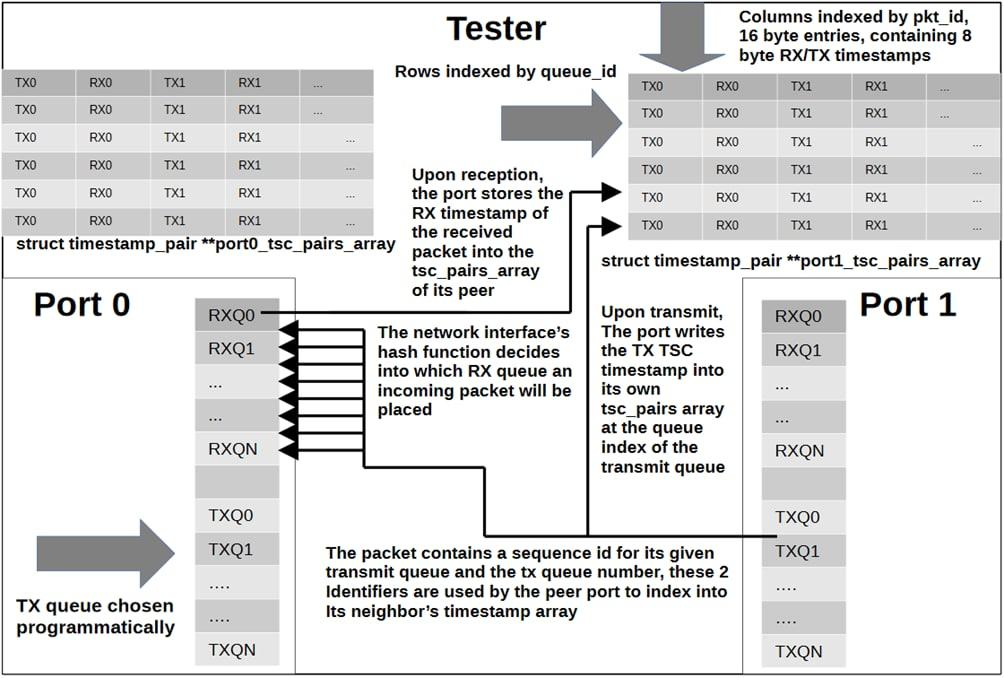
\includegraphics[width=\textwidth]{6transperfarchitecture}


The pkt\_id and queue\_id are extracted during the receive path:

\begin{frame}

\lstset{language=C++,breaklines=true,numbers=left}
\begin{lstlisting}
        if (timestamp_all_packets) {
                uint64_t qnum, pktid;
                if (port0->m_config->is_ipip6_tun_intf) {
                        qnum = extract_ipip6_queue_id(buf);
                        pktid = extract_ipip6_pkt_id(buf);
                } else {
                        qnum  = extract_ip_queue_id(buf);
                        pktid = extract_ip_queue_id(buf);
                }
             port0_tsc_pairs_array[qnum][pktid].rx_tsc_value=received_tsc;
        }
\end{lstlisting}
\end{frame}

The functions for extracting the pkt\_id, and queue\_ids and for verifying that the current frame is a test frame are simple functions reading into specific offsets of the received mbuf:

\begin{frame}

\lstset{language=C++,breaklines=true,numbers=left}
\begin{lstlisting}

inline uint64_t extract_ipip6_queue_id(char *buf)
{
        uint64_t *data = (uint64_t *) (buf+
                        (sizeof(struct ether_hdr))+
                        (sizeof(struct ipv6_hdr))+
                        (sizeof(struct ip6_opt))+
                        (sizeof(struct ip6_opt_tunnel))+
                        (sizeof(struct ip6_opt_padn))+
                        (sizeof(struct ipv4_hdr))+
                        (sizeof(struct udp_hdr)) + 16);

        return *data;
}

\end{lstlisting}
\end{frame}

\subsection{Tests and results:}

In the table below we have gathered the results from 20 experiments uing 64, 512 and 1512 byte frames. From the 20 experiments the Median, 1st and 99th percentile is listed: 

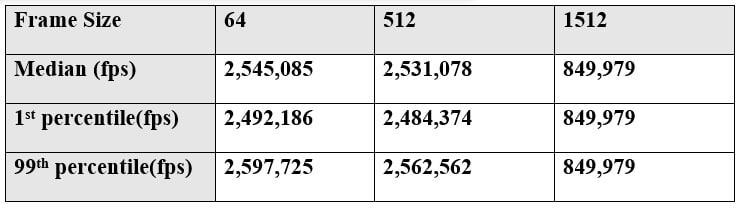
\includegraphics[width=\textwidth]{results}

\subsection{Discussion of results:}
It can be observed that a ceiling has been reached regarding how any frames per second we are able to send, it is believed that once 6transperf implements the randomized port feature according to RFC4814 this ceiling can be overcome.
\subsection{Conclusion:}
6transperf is still in active development, the functionality it supports today is extremely limited, however the aims to become the first DS-Lite tester conforming to RFC8219 is projected to be fulfilled early 2022.
\end{document}